%%%%%%%%%%%%%%%%%%%%%%%%%%%%%%%%%%%%%%%%%%%%%%%%%%%%%%%%%%%%%%%%%%%%%%%%%%%%%%%%%
%%%%%                           EXPERIENCED MW                               %%%%
%%%%%%%%%%%%%%%%%%%%%%%%%%%%%%%%%%%%%%%%%%%%%%%%%%%%%%%%%%%%%%%%%%%%%%%%%%%%%%%%%

Thus far we have used the statutory minimum wage as our variable of interest (i.e., 
the maximum across federal, state and local levels). While this variable correctly 
captures the underlying relevant increase in income across low-wage workers for large
geographical areas, such as states, it is likely to be less precise at the local level,as 
individuals commute across zipcodes. As discussed throughout the paper, a central feature of MW 
policies is the geographical scope inherently associated with them. Hence, accounting 
for workplace and residence locations of low-wage workers can provide valuable insight 
into the question of how MW changes affect the housing market. 

The underlying assumptions behind this view are that rents are determined by the 
intersection of rental housing supply and demand, and that demand is
positively associated with income. As a result, we would expect MW policies to increase 
rents in neighborhoods where low-wage workers live, since those experience a positive
income shock due to the policy. On the other hand,  in zipcodes with a low share 
of MW residents we may expect a small or insignificant income shock, especially 
in the short-run (\cite{allegretto2018local} suggest how the whole MW increase in 
the restaurant industry is passed to consumers via prices. In such case, lower 
restaurant consumption may actually lead to decreasing rents.). 
As a matter of fact, the heterogeneity analysis in 
\autoref{sec:heter} suggests that the effect is stronger in zipcodes with a high
concentration of low-wage workers. We explore this possibility more deeply in this 
section.

We begin by discussing features of the experienced MW measure, 
introduced in \autoref{sec:data}, and comparing it with the statutory MW. 
We use this measure in two ways. First, we use it as dependent variable in our main models, 
and find that the estimated elasticity slightly increases. Second, ... COMPLETE

%%%%%%%%%%%%%%%%%%%%%%%%%%%%%%%%%%%%%%%%%%%%%%%%%%%%%%%%%%%%%%%%%%%%%%%%%%%%%%%%%
\subsection{A New Minimum Wage Measure}

As shown in the heterogeneity analysis of \autoref{sec:heter}, the effect of MW policies 
appears to be stronger for zipcodes with a higher concentration of MW residents. This 
provides an empirical justification for refining the main explanatory variable so to 
better account for the fact that residence and workplace of workers tends to diverge, 
and that MW policies in the latter determine low-wage workers' income. As explained in 
\autoref{sec:mw_construction}, we compute the experienced MW for a given zipcode $i$ as 
the weighted average of the statutory MW in zipcodes where $i$'s residents  work.
The weight for each origin-destination pair is the share of the origin workforce commuting to
the destination zipcode. weights correspond to the share of the workforce in $i$ that works in 
each destination zipcode in the LODES data.

\autoref{fig:expmw_san_diego} illustrates the difference between our MW measures by plotting 
the percent change in statutory and experienced MW variables following the California 
increase of January 2019. As of December 2018 the MW in San Diego city was \$11.50, 
whereas the state's MW binding outside the city was \$11.\footnote{For employers larger 
	than 26 employees. For those below 26 employees the level was \$10.50. As explained in 
	\autoref{sec:data}, our variable uses the statutory MW variable takes the MW for
	large employers in this case. [WE EXPLAIN THIS? CHECK]}
The increase in the state level MW to \$12 in January 2020 appears as a discontinuity in the 
city border. However, when we account for the fact that MW workers commute, we observe a 
gradient in the intensity of the policy.

\begin{figure}
	\caption{The California MW Increase of January 2019 in San Diego}
	\label{fig:expmw_san_diego}
	\centering
	\begin{subfigure}[b]{0.65\textwidth}
		\caption{Statutory MW change}
		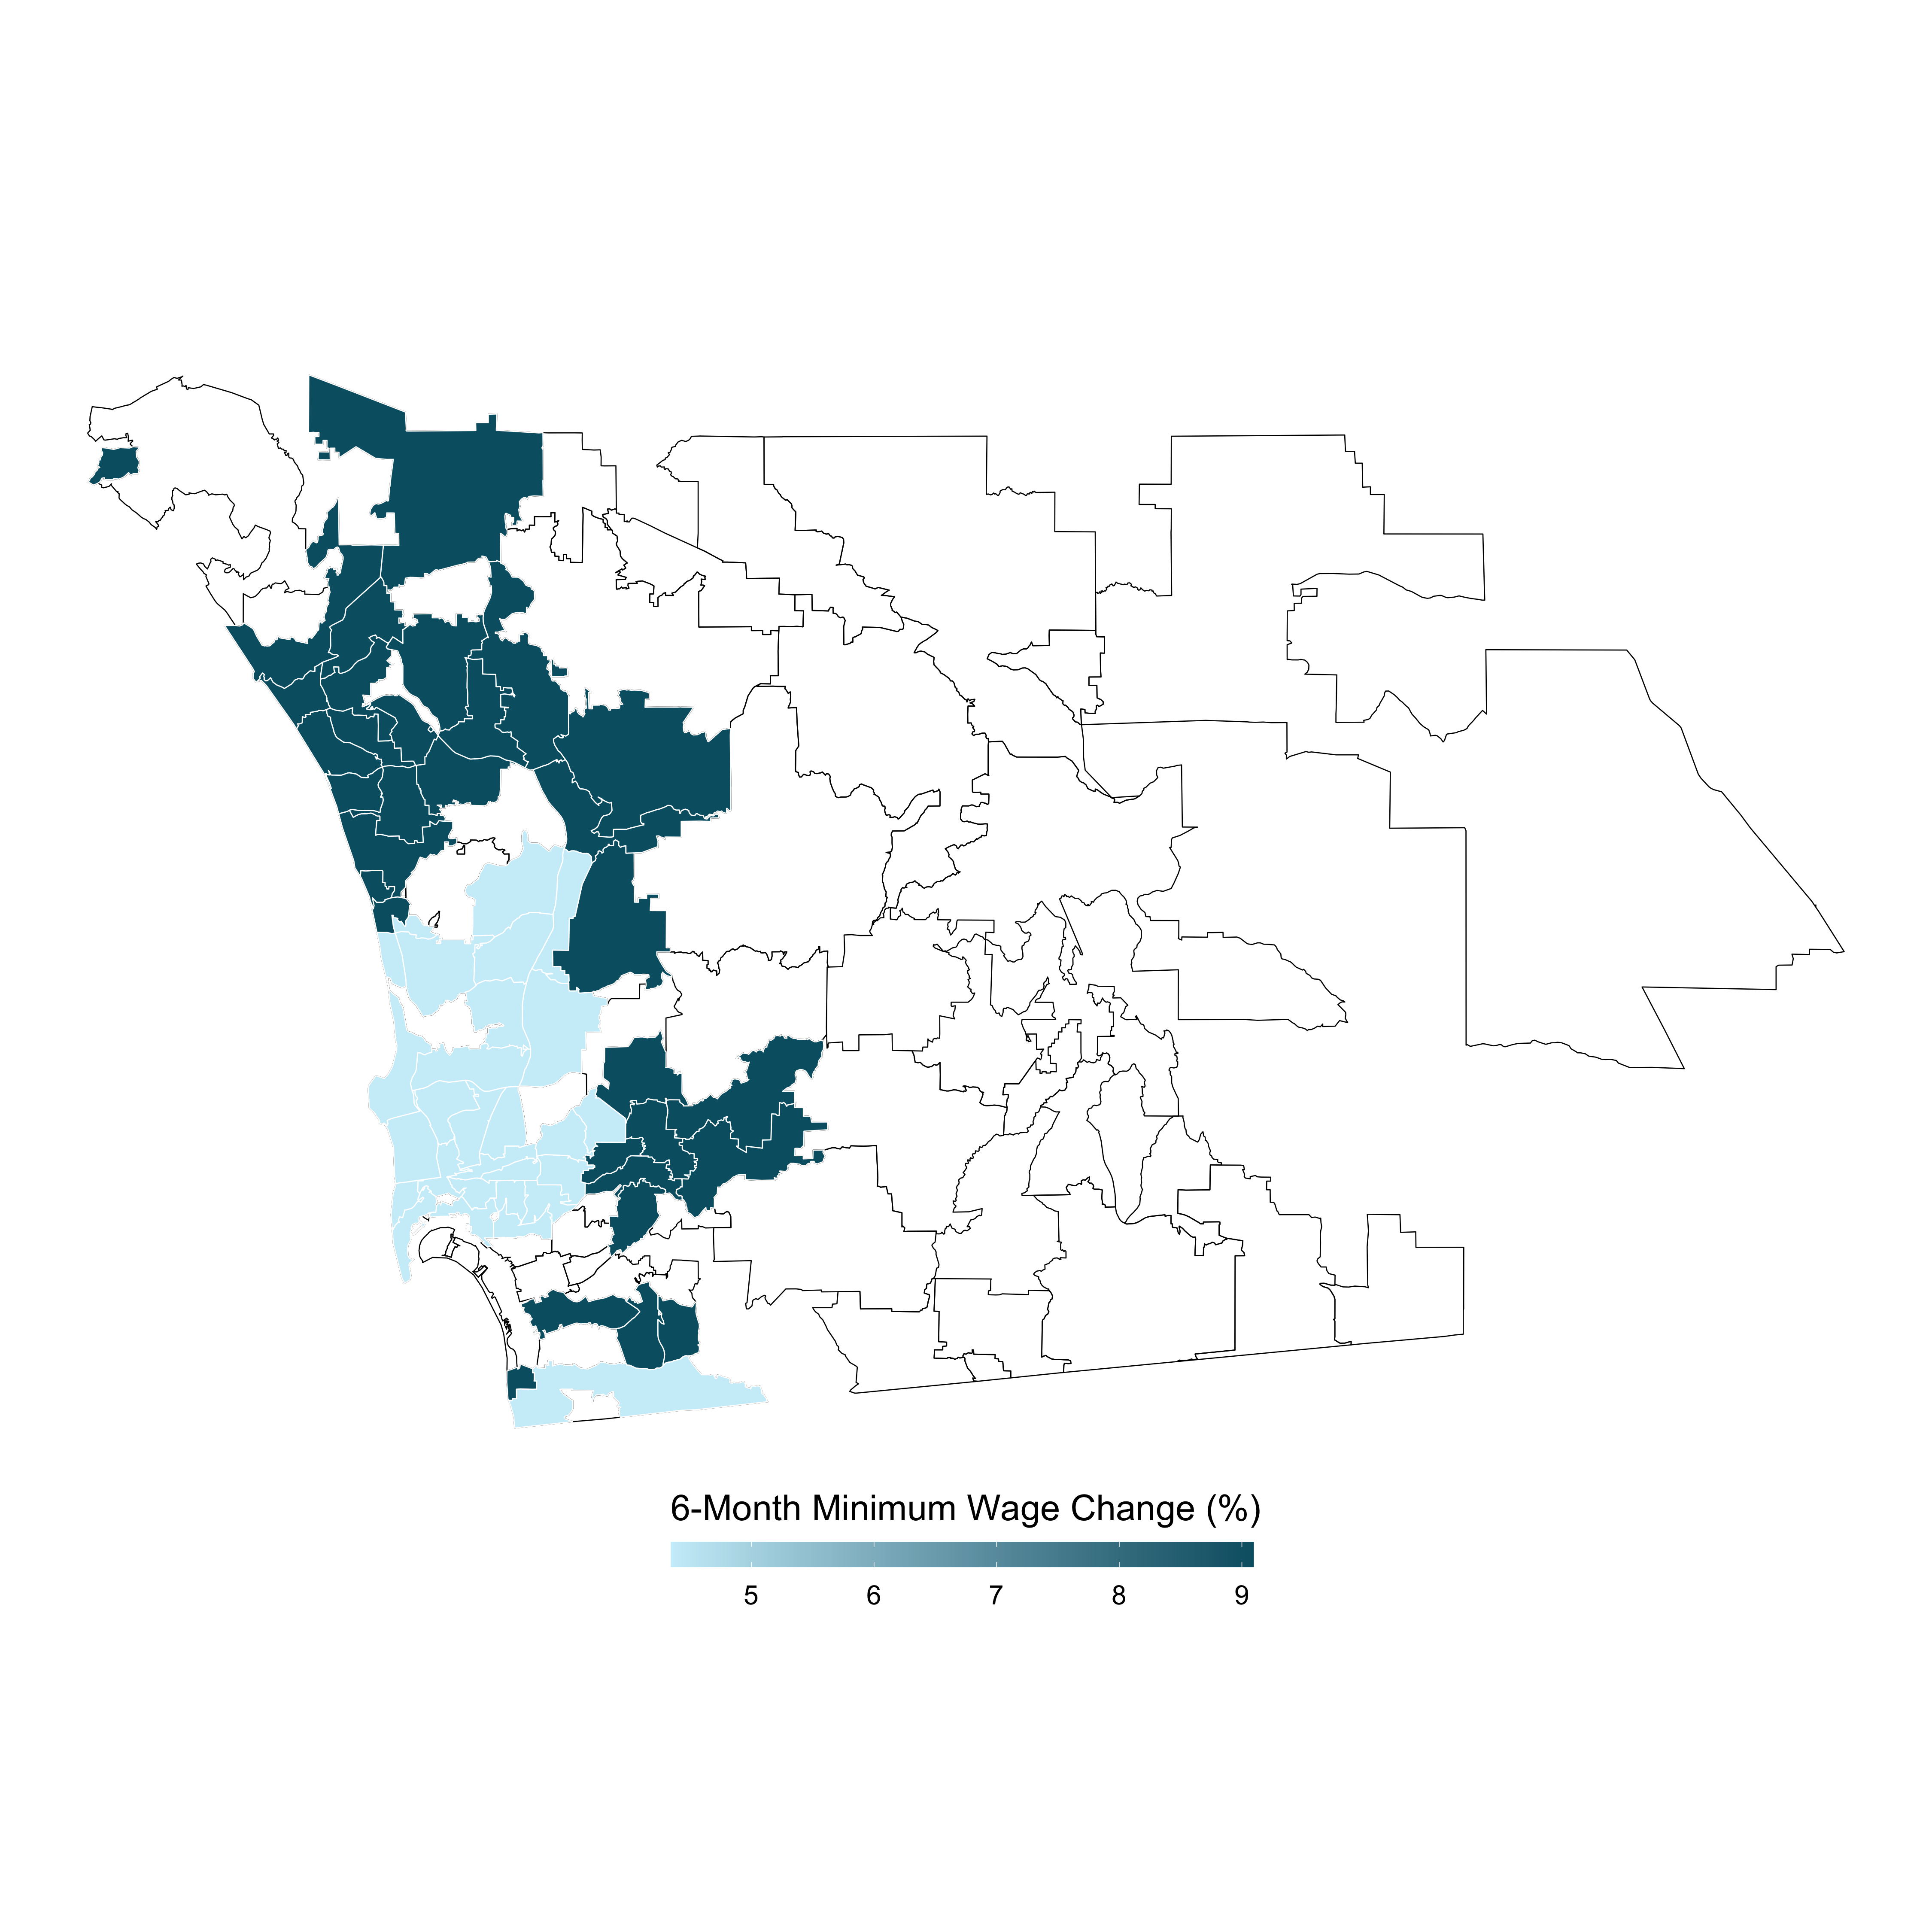
\includegraphics[width = \textwidth]
		{../../analysis/descriptive_maps/output/San_Diego_mw_msa.png}
	\end{subfigure}\\
	\begin{subfigure}[b]{0.65\textwidth}
		\caption{Experienced MW change}
		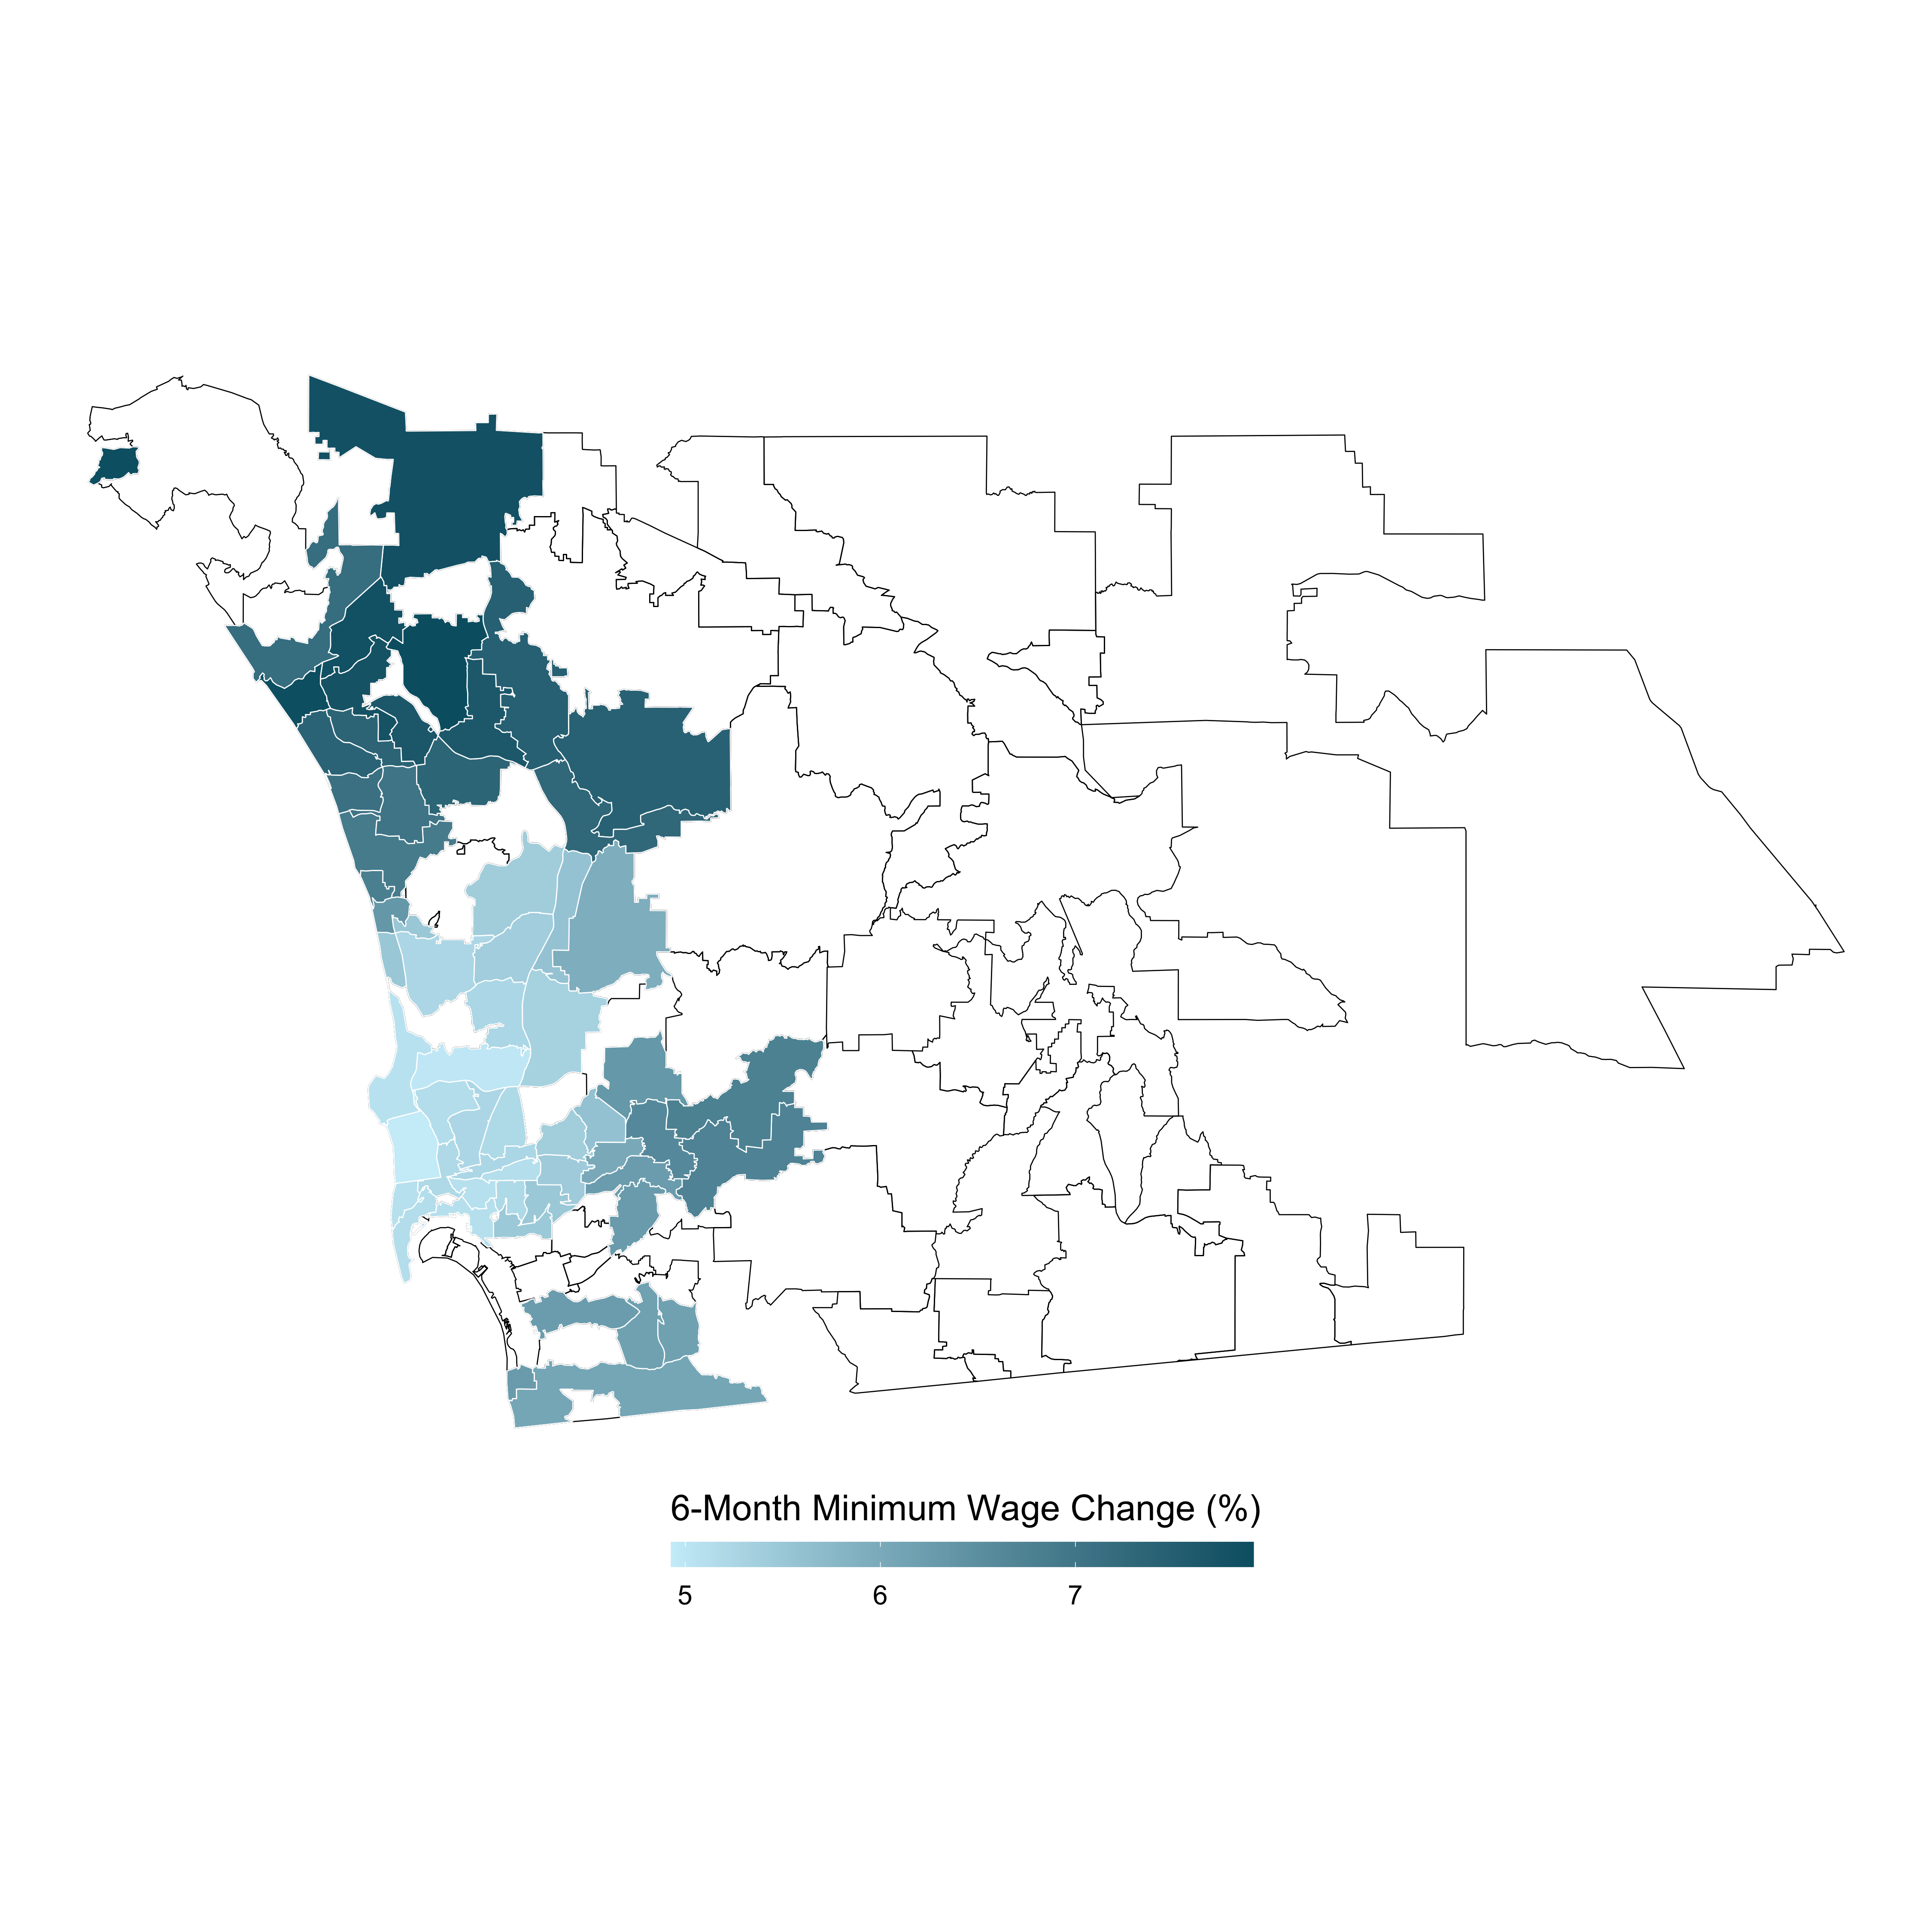
\includegraphics[width = \textwidth]
		{../../analysis/descriptive_maps/output/San_Diego_expmw_msa.png}
	\end{subfigure}
	\begin{minipage}{0.95\textwidth} \footnotesize
		\vspace{2mm} 
		\textit{Notes}: The figure maps the percent increase in our minimum wage and 
		experienced minimum wage measures following the state increase in California
		on January 2019. The map colors only those zipcodes for which we have 
		non-missing rents data from Zillow.
	\end{minipage}
\end{figure}

The new measure we obtain is highly correlated with the original statutory MW. The 
correlation in the levels of the variables is 0.985, whereas the correlation between the 
difference of natural logarithms is 0.971. %% Document in repo
However, these variables are not identical, and they show an important degree of independent 
variation. To see this, first note that our experienced MW results in a larger number of 
treated zipcode-month observations in our baseline panel, increasing the number of events 
from 5,302 to 8,942. %% Document in repo
Hence, there are 3,640 zipcode-month cells that went from being zero to a positive value. 
The variables not only differ in the number of non-zero changes, but also in their intensity. 
The first column of \autoref{tab:expmw_main} reports the results of running our main static 
model but using the change in the experienced MW $\Delta \ln \underline{w}_{itc}^{\text{exp}}$ 
as dependent variable. After conditioning on zipcode and time period fixed effects
and our preferred set of economic controls, we observe that, on average, a 1 percent increase 
in the statutory MW translates into a 0.89 percent increase in the experienced MW. This 
regression suggests that the measures have more independent variation than suggested by 
raw correlations alone.

Where does that independent 
variation originate? State-wide MW increases are unlikely to induce it, since they tend to 
affect near-by zipcodes in a similar fashion. Local MW policies (either at the county or city
levels) are the obvious candidates, since they usually affect zipcodes in close proximity 
differentially. Appendix \autoref{fig:residu_expmw} shows that this is indeed the case. 
There we take the residuals from the regression in the first column of 
\autoref{tab:expmw_main}, we compute their standard deviation within zipcodes, and we plot 
them against the number of events in those zipcodes. As suggested by the OLS fit, the residuals
tend to vary more in places that had many local events, whereas the standard deviation is not 
correlated to state events. This suggests how the two measures will generally differ whenever the 
zipcodes' commuting area does not overlap with the jurisdictional level enacting the MW 
policy. We interpret this evidence as indication that variation in the 
experienced MW that is uncorrelated with the statutory one arises particularly from local 
events.\footnote{Formally, the estimated model is 
	$$ \Delta \ln \underline{w}_{itc}^{\text{exp}} = \delta_t 
				+ \beta \Delta \ln \underline{w}_{ict} + \Delta \mathbf{X}^{'}_{ct} \eta 
				+ \Delta \nu_{ict} . $$
	By definition, $\Delta \nu_{ict}$ is uncorrelated with $\Delta \ln \underline{w}_{ict}$ 
	conditional on the controls. The presence of enough variation in these residuals allows us
	to identify a regression on rents including both MW measures as controls, discussed in the
	next section.}


%%%%%%%%%%%%%%%%%%%%%%%%%%%%%%%%%%%%%%%%%%%%%%%%%%%%%%%%%%%%%%%%%%%%%%%%%%%%%%%%%
\subsection{Estimation Results}
\begin{table}[htb!]\centering
	\caption{The Impact of Experienced Minimum Wage Changes on Rents}
	\label{tab:expmw_main}
	{
\def\sym#1{\ifmmode^{#1}\else\(^{#1}\)\fi}
\begin{tabular}{l*{4}{c}}
\hline\hline
          &\multicolumn{1}{c}{$\Delta \underline{w}_{ict}^{\text{exp}}$}&\multicolumn{3}{c}{$\Delta \ln r_{ict}$}                \\\cmidrule(lr){2-2}\cmidrule(lr){3-5}
          &\multicolumn{1}{c}{(1)}         &\multicolumn{1}{c}{(2)}         &\multicolumn{1}{c}{(3)}         &\multicolumn{1}{c}{(4)}         \\
\hline
$\Delta \ln \underline{w}_{ict}$&   0.8718\sym{***}&   0.0257\sym{*}  &                  &  -0.0320\sym{*}  \\
          & (0.0296)         & (0.0137)         &                  & (0.0163)         \\
[1em]
$\Delta \underline{w}_{ict}^{\text{exp}}$&                  &                  &   0.0320\sym{**} &   0.0662\sym{**} \\
          &                  &                  & (0.0151)         & (0.0278)         \\
\hline
$\Delta \ln \underline{w}_{ict}$ + $\Delta \underline{w}_{ict}^{\text{exp}}$&                  &                  &                  &                  \\
          &                  &                  &                  &                  \\
\vspace{-2mm}&                  &                  &                  &                  \\
Wage controls&      Yes         &      Yes         &      Yes         &      Yes         \\
Employment controls&      Yes         &      Yes         &      Yes         &      Yes         \\
Establishment-count controls&      Yes         &      Yes         &      Yes         &      Yes         \\
P-value equality&                  &                  &                  &    0.027         \\
R-squared &    0.947         &    0.021         &    0.021         &    0.021         \\
Observations&  131,196         &  131,196         &  131,196         &  131,196         \\
\hline\hline
\end{tabular}
}

	\begin{minipage}{0.95\textwidth}\footnotesize
		\vspace{3mm}	
		\textit{Notes:} The table shows versions of the static model using different 
		dependent and MW variables. Column 1 shows a regression of the change in the natural 
		logarithm of the experienced MW on the change in the natural logarithm of the 
		statutory MW. Column 2, 3, and 4 use the change natural logarithm of median rents per 
		square foot in the SFCC category as dependent variable. Column 2 uses the change in 
		the natural logarithm of the statutory MW, column 3 uses the change in the natural 
		logarithm of the experienced MW, and column 4 uses both. All models control for time 
		period fixed effects and, additionally, for our preferred set of economic controls 
		from the QCEW. 
		Standard errors clustered at the state level are reported in parenthesis. Significance 
		codes: *** $p < 0.01$, ** $p < 0.05$, * $p < 0.1$.
	\end{minipage}
\end{table}

In this section we re-estimate our main models using the experienced MW. As discussed in 
\autoref{sec:emp_strategy_expmw}, an initial way to use this new measure is to directly
replace the statutory MW changes in the static and dynamic regression models. 
Under the plausible assumption that income and rent are correlated in local 
housing markets, then the experienced MW better capture the relevant level of the 
MW for determining incomes in a zipcode.In this case, classical measurement error 
arguments imply that the experienced MW effect should generate a stronger impact on rents. 

We explore this possibility in columns 2 to 4 in \autoref{tab:expmw_main}. Column 2 
shows our baseline static model, in which the elasticity of rents per square foot is 
estimated to be 0.026 (s.e. 0.012). Column 3 reports the same model when using the 
experienced MW as main explanatory variable. The static effect increases slightly, to 0.031 (s.e. 0.013).
While it is true that this coefficients are statistically indistinguishable, the results
confirm the presence of a small attenuation bias in baseline models. 
Appendix \autoref{fig:expmw_dynamic} compares the dynamic models when using either MW 
measure, and similarly suggests that the cumulative effect is slightly larger when using
the experienced MW.

A second and arguably more interesting exercise consists of including both MW measures in
the same static model. As argued in the previous section, these measures show significant
independent variation to allow for identification of both coefficients of such model. 
Column 4 of \autoref{tab:expmw_main} reports the results. The statutory MW induces
a slight \textit{decrease} in rents, with a point estimate of $-$0.027 (s.e. 0.02). The 
experienced MW, on the other hand, shows a strong positive effect of rents with a 
coefficient of 0.059 (s.e. 0.028), twice as large as the point estimate in Column 3. We
conducted an F-stat for the equality of both coefficients in Column 4, which rejects the
null hypothesis of equality at the 10\% significance level (p-value 0.075). 
% See first_differences_expmw/output/test_coefficients_static.log

We see these results as suggestive evidence of a supply and demand mechanism driving the 
effects. Conditional on the reasonable assumptions that the demand for rental units determines 
local rents, and such demand is increasing in income, then a MW policy introduces a income transfer 
from zipcodes in which low-wage workers work to those where they reside (conditional on 
small disemployment effects). That is because the price of local consumption in richer zipcodes must go up 
to afford the increased cost of low-wage labor \parencite{allegretto2018local}. 
As a result, real incomes of residents of richer zipcodes will go down, impacting negatively median 
rents there. In contrast, real incomes
of zipcodes with many low-wage residents will increase, translating into higher rents. 
We think that the inclusion of the actual and experienced MW measures are capturing precisely
that variation.


